\section{Persistenz}

\begin{concept}{Persistenz Grundlagen}\\
Persistenz bezeichnet die dauerhafte Speicherung von Daten über das Programmende hinaus:
\begin{itemize}
    \item Speicherung in Datenbankmanagementsystemen (DBMS)
    \item Haupttypen:
    \begin{itemize}
        \item Relationale Datenbanksysteme (RDBMS)
        \item NoSQL-Datenbanken (ohne fixes Schema)
    \end{itemize}
    \item O/R-Mapping (Object Relational Mapping)
    \begin{itemize}
        \item Abbildung zwischen Objekten und Datensätzen
        \item Überwindung des Strukturbruchs (Impedance Mismatch)
    \end{itemize}
\end{itemize}
\end{concept}

\begin{definition}{O/R-Mismatch}\\
Der Strukturbruch zwischen objektorientierter und relationaler Welt:
\begin{itemize}
    \item \textbf{Typen-Systeme:}
    \begin{itemize}
        \item Unterschiedliche NULL-Behandlung
        \item Datum/Zeit-Darstellung
    \end{itemize}
    \item \textbf{Beziehungen:}
    \begin{itemize}
        \item Richtung der Beziehungen
        \item Mehrfachbeziehungen
        \item Vererbung
    \end{itemize}
    \item \textbf{Identität:}
    \begin{itemize}
        \item OO: Implizite Objektidentität
        \item DB: Explizite Identität (Primary Key)
    \end{itemize}
\end{itemize}
\end{definition}

\subsection{JDBC - Java Database Connectivity}

\begin{concept}{JDBC Grundlagen}\\
JDBC ist die standardisierte Schnittstelle für Datenbankzugriffe in Java:
\begin{itemize}
    \item Seit JDK 1.1 (1997)
    \item Plattformunabhängig
    \item Datenbankunabhängig
    \item Aktuelle Version: 4.2
\end{itemize}
\end{concept}

\begin{KR}{JDBC Verwendung}
Grundlegende Schritte für Datenbankzugriff:
\begin{enumerate}
    \item JDBC-Treiber installieren und laden
    \item Verbindung zur Datenbank aufbauen
    \item SQL-Statements ausführen
    \item Ergebnisse verarbeiten
    \item Transaktion abschließen (Commit/Rollback)
    \item Verbindung schließen
\end{enumerate}
\end{KR}



\subsection{Design Patterns für Persistenz}

\begin{theorem}{Persistenz Design Patterns}\\
Drei grundlegende Ansätze für die Persistenzschicht:
\begin{itemize}
    \item \textbf{Active Record (Anti-Pattern):}
    \begin{itemize}
        \item Entität verwaltet eigene Persistenz
        \item Vermischung von Fachlichkeit und Technik
        \item Schlechte Testbarkeit
    \end{itemize}
    \item \textbf{Data Access Object (DAO):}
    \begin{itemize}
        \item Kapselung des Datenbankzugriffs
        \item Trennung von Fachlichkeit und Technik
        \item Gute Testbarkeit durch Mocking
    \end{itemize}
    \item \textbf{Repository (DDD):}
    \begin{itemize}
        \item Abstraktionsschicht über Data-Mapper
        \item Zentralisierung von Datenbankabfragen
        \item Komplexere Implementierung
    \end{itemize}
\end{itemize}
\end{theorem}

\begin{KR}{DAO Implementation}\\
Schritte zur Implementierung eines DAOs:
\begin{enumerate}
    \item Interface definieren:
    \begin{itemize}
        \item CRUD-Methoden (Create, Read, Update, Delete)
        \item Spezifische Suchmethoden
    \end{itemize}
    \item Domänenklasse erstellen:
    \begin{itemize}
        \item Nur fachliche Attribute
        \item Keine Persistenzlogik
    \end{itemize}
    \item DAO-Implementierung:
    \begin{itemize}
        \item Datenbankzugriff kapseln
        \item O/R-Mapping implementieren
        \item Transaktionshandling
    \end{itemize}
\end{enumerate}
\end{KR}



\subsection{Java Persistence API (JPA)}

\begin{concept}{JPA Grundkonzepte}\\
JPA ist der Java-Standard für O/R-Mapping:
\begin{itemize}
    \item \textbf{Entity-Klassen:}
    \begin{itemize}
        \item Plain Old Java Objects (POJOs)
        \item Annotation @Entity
        \item Keine JPA-spezifischen Abhängigkeiten
    \end{itemize}
    \item \textbf{Referenzen:}
    \begin{itemize}
        \item Eager/Lazy Loading
        \item Automatisches Nachladen
    \end{itemize}
    \item \textbf{Provider:}
    \begin{itemize}
        \item Hibernate
        \item EclipseLink
        \item OpenJPA
    \end{itemize}
\end{itemize}
\end{concept}

\begin{concept}{JPA Technologie-Stack}\\
\begin{itemize}
    \item Java Application
    \item Java Persistence API
    \item JPA Provider (Hibernate, EclipseLink, etc.)
    \item JDBC Driver
    \item Relationale Datenbank
\end{itemize}
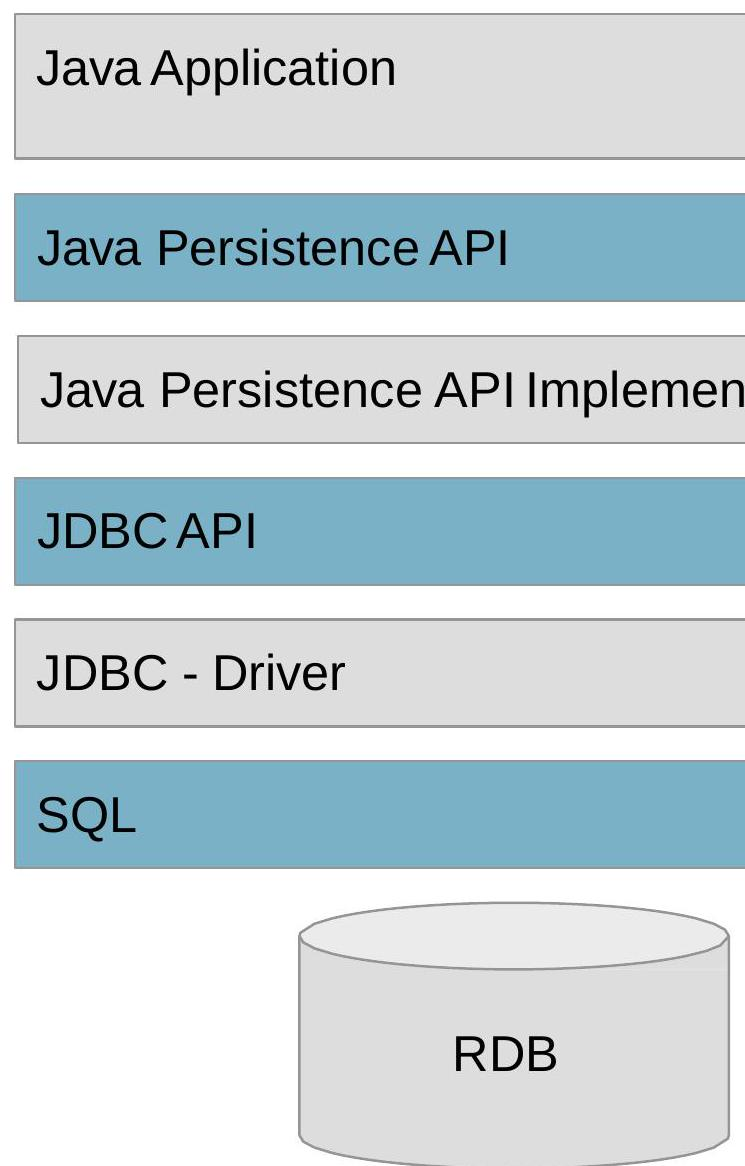
\includegraphics[width=0.8\linewidth]{images/2025_01_02_5ba1dc702e9f94ba8e06g-29.jpg}
\end{concept}

\begin{KR}{JPA Entity Erstellung}
\begin{enumerate}
    \item Entity-Klasse definieren:
    \begin{itemize}
        \item @Entity Annotation
        \item ID-Feld mit @Id markieren
    \end{itemize}
    \item Beziehungen definieren:
    \begin{itemize}
        \item @OneToMany, @ManyToOne etc.
        \item Navigationsrichtung festlegen
    \end{itemize}
    \item Validierung hinzufügen:
    \begin{itemize}
        \item @NotNull, @Size etc.
        \item Geschäftsregeln
    \end{itemize}
\end{enumerate}
\end{KR}



\subsection{Repository Pattern}

\begin{concept}{Repository Pattern}\\
Das Repository Pattern bietet eine zusätzliche Abstraktionsschicht über der Data-Mapper-Schicht:
\begin{itemize}
    \item Zentralisierung von Datenbankabfragen
    \item Domänenorientierte Schnittstelle
    \item Unterstützung komplexer Abfragen
    \item Häufig in Kombination mit Spring Data
\end{itemize}
\end{concept}



\begin{remark}
Spring Data unterstützt die automatische Generierung von Repository-Implementierungen basierend auf Methodennamen. Dies reduziert den Implementierungsaufwand erheblich.
\end{remark}